% !TEX root = ../finalReport.tex
% "What is the current state of computer science regarding games like Nonaga?"
\chapter{Introduction and Background Research}

% You can cite chapters by using '\ref{chapter1}', where the label must
% match that given in the 'label' command, as on the next line.
\label{chapter1}

% Sections and sub-sections can be declared using \section and \subsection.
% There is also a \subsubsection, but consider carefully if you really need
% so many layers of section structure.

\section{Project Aim}
\label{sec:aim}

The primary aim of this project is to architect and develop a high-performance computer program capable of playing the board game Nonaga at a highly competitive level. While playing a board game is intuitively simple for humans, teaching a machine to do so requires solving complex computational challenges.

To achieve this overarching aim, the project focuses on several core objectives, designed to tackle the problem from a high-level computational perspective:

\begin{itemize}
  \item \textbf{Engine Optimization (The Board Representation):} Before an AI can play, it must understand the board efficiently. A major objective is to design a highly optimized internal representation of the game. This foundational layer must process rules and generate possible moves almost instantaneously, ensuring the AI can operate at high speeds without performance drag.

  \item \textbf{Adversarial Search (Looking Ahead):} The AI needs the ability to predict future outcomes. This objective involves implementing a strategic decision-making algorithm that allows the system to simulate thousands of potential future board states. By evaluating these outcomes, the system can quickly discard mathematically poor moves and select the most advantageous ones.

  \item \textbf{Evaluation Optimization (Developing Intuition):} The AI must be able to judge whether each board positions are advantageous. To implement this "intuition," the project implements an automated learning framework. By having the AI play thousands of simulated matches, the system systematically evolves and improves itself without relying on human intervention.

  \item \textbf{Interactive Client Development (User Interface):} To make the engine accessible and testable, the final objective is building a simple Graphical User Interface (GUI) that allows human users to play against the AI.

\end{itemize}


\section{Introduction to Nonaga and the Computational Problem}
% Explain Nonaga briefly to a non-expert. 
% Pivot to the computational bottleneck: high branching factor and connectivity checking.
\subsection{What is Nonaga?}
Nonaga is an abstract strategy board game created by Viktor Bautista i Roca that opposes two players playing as Red and Black \cite{nonaga_rules}. The primary objective is straightforward: a player wins by manoeuvring their three individual circular pieces so that they connect and form a single continuous group as shown in \cref{fig:win_configs}. \\



\begin{figure}[H]
  \centering
  \begin{subfigure}{0.3\textwidth}
    \centering
    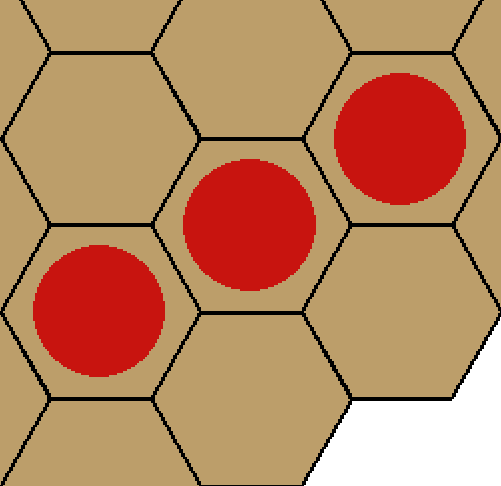
\includegraphics[width=0.7\textwidth]{pictures/Nonaga_intro/line win.png}
    \caption{Line Configuration}
    \label{subfig:line_win}
  \end{subfigure}\hfill
  \begin{subfigure}{0.3\textwidth}
    \centering
    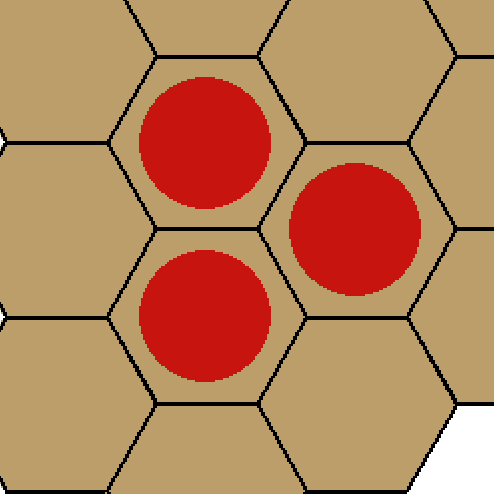
\includegraphics[width=0.7\textwidth]{pictures/Nonaga_intro/triangle win.png}
    \caption{Triangle Configuration}
    \label{subfig:triangle_win}
  \end{subfigure}\hfill
  \begin{subfigure}{0.3\textwidth}
    \centering
    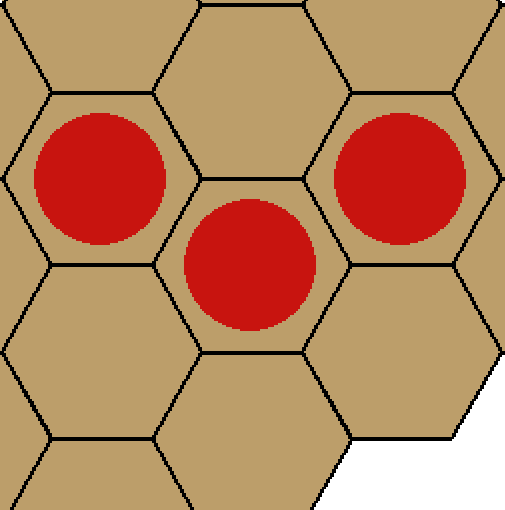
\includegraphics[width=0.7\textwidth]{pictures/Nonaga_intro/curve win.png}
    \caption{Curve Configuration}
    \label{subfig:curve_win}
  \end{subfigure}

  \caption{The three winning configuration shapes for Red.}
  \label{fig:win_configs}
\end{figure}


The game is played on a dynamically shifting board composed of 19 independent hexagonal tiles. The structure of a turn consists of two distinct mandatory phases. First, a player must slide one of their pieces in a straight line; the piece cannot stop voluntarily and must continue moving until it collides with another piece or reaches the edge of the board (\cref{subfig:piece_move}). Second, the player must alter the playing area itself by removing an unoccupied tile from the outer edge of the board and reattaching it to a different valid location on the perimeter (\cref{subfig:tile_move}). An example game played between two human players can be found in \cite{nonaga_demo_2026}. Not all tiles can be moved in every position, the rules of tile movability are further explained in \cref{sec:tile_movement_legality}.\\


\begin{figure}[H]
  \centering
  \begin{subfigure}{0.43\textwidth}
    \centering
    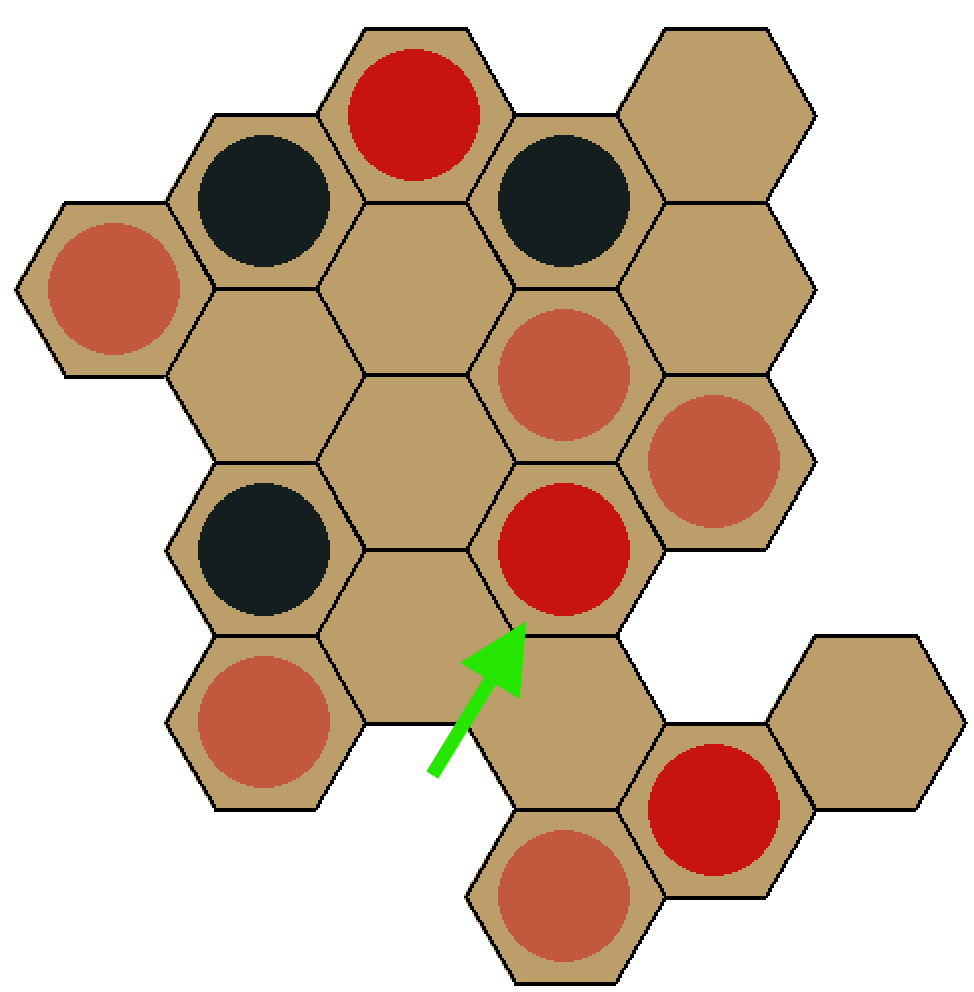
\includegraphics[width=\textwidth]{pictures/Nonaga_intro/Piece move.png}
    \caption{Legal destinations for the piece pointed to by the green arrow shown in light red.}
    \label{subfig:piece_move}
  \end{subfigure}\hfill
  \begin{subfigure}{0.43\textwidth}
    \centering
    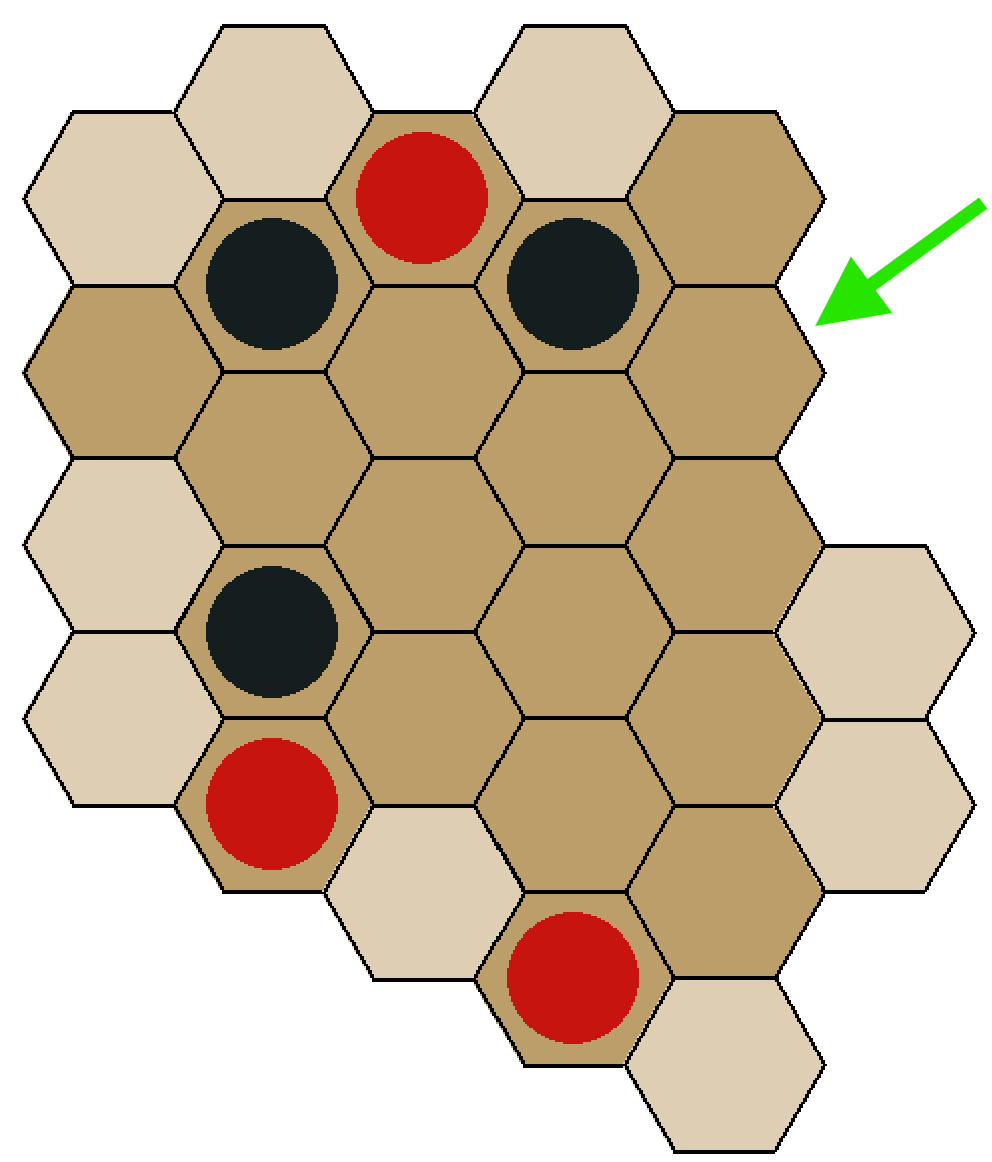
\includegraphics[width=\textwidth]{pictures/Nonaga_intro/Tile move.png}
    \caption{Legal destinations for the tile pointed to by the green arrow shown in light brown.}
    \label{subfig:tile_move}
  \end{subfigure}

  \caption{Piece and tile movement examples.}
  \label{fig:player_moves}
\end{figure}


Although these mechanics are intuitive for a human player, this two-phase turn structure introduces severe computational complexity. Because a single turn requires both a piece movement and a tile movement which alters the structure of the board, the number of possible legal moves available at any given moment, is exceptionally high (estimated at~440 in \cref{branching}).

Moreover, the state of the board requires continuous recomputation; between each turn, the legality of moving any specific tile must be dynamically evaluated based on the connectivity of its immediate neighbours.\\

Furthermore, to the best of our knowledge, there is currently no published academic literature addressing Nonaga.


\section{Board State Representation}

\subsection{Hexagonal Coordinate Systems}\label{sec:hex_coord}

Before establishing a board state representation, a fundamental design decision is the selection of a hexagonal coordinate system, as this choice directly governs the algebraic complexity of neighbour lookup, distance calculation, and direction traversal. Three primary systems are documented in the literature \cite{patel2013hexagons, 8848436}:
\begin{itemize}

  \item Offset coordinates adapt the familiar square grid by shifting alternate rows or columns by half a cell width. While immediately intuitive, this system introduces an asymmetry: the direction vectors required to reach a neighbour differ depending on whether the current cell occupies an even or odd row, complicating the implementation of uniform geometric algorithms.

  \item Cube coordinates embed the hexagonal plane in three-dimensional space on the constraint surface $x + y + z = 0$, yielding uniformly simple distance and rotation formulae via unit-step axis permutations. The cost is a redundant third coordinate that must be carried and validated throughout all computations.

  \item Axial coordinates derive directly from cube coordinates by exploiting the linear constraint to eliminate the third axis, retaining only two values $(q, r)$. This preserves the uniform neighbour structure and constant direction vectors of the cube system while reducing the representational overhead, and produces a particularly clean mapping from hexagonal geometry onto linear memory structures \cite{patel2013hexagons}.

\end{itemize}
\subsection{Object-Oriented Representation}

The most straightforward approach for board state representation is Object-Oriented Design (OOD), which instantiates discrete game entities as classes. While this method accelerates initial development and aligns with human conceptual models of a board game, OOD struggles to efficiently utilize computing resources in performance-critical applications \cite{wingqvist2022dod}. Because objects are dynamically allocated, they become scattered across system memory. During the millions of rapid state evaluations required by an Artificial Intelligence (AI) search algorithm, this lack of spatial locality leads to severe CPU cache misses and memory latency, severely bottlenecking engine performance \cite{arantes2025impact}.

\subsection{Bitboard Representation}

On the opposite, modern high-performance engines rely on Data-Oriented Design (DOD), which prioritizes memory contiguity and hardware-level efficiency. By representing the game state as a series of 64-bit integers, known as "bitboards", the engine can map boolean states (e.g., piece presence, color, or valid tiles) directly to individual bits. Studies have shown that contiguous, bit-level representations can achieve speedups of over 13x compared to equivalent OOP architectures by maximizing cache efficiency and allowing parallel evaluations via bitwise logical operations (AND, OR, XOR) \cite{wingqvist2022dod}.

While bitboards are the de facto standard in computer chess, they present unique implementation paradigms that must be carefully evaluated. Bitboard state transitions can theoretically operate 64 times faster than array encodings; however, poorly optimized bit-manipulation can introduce significant overhead, making the underlying mathematical model critical \cite{segundo2006}. Furthermore, generalizing bitboards to non-standard geometries requires careful mathematical mapping \cite{browne2014bitboards}.

\subsubsection{Evaluating Bitboard Architectures for Sliding Pieces}

A fundamental challenge in bitboard design is move generation, which is broadly categorized into "leaping" and "sliding" mechanics \cite{browne2014bitboards}. Leaping pieces (such as a Knight in chess) have static attack patterns relative to their coordinate, requiring a simple array lookup: \texttt{Attacks[coordinate]}.

Conversely, sliding pieces, which move continuously along an axis until obstructed by the board edge or another piece, require dynamic calculation based on current board occupancy. Historically, computing these sliding rays using step-by-step bitwise shifts was computationally expensive \cite{hyatt1999rotated}. To mitigate this, two primary architectures used for chess have dominated engine design:

\begin{itemize}

  \item \textbf{Rotated Bitboards:} An older, slower technique that maintains multiple redundant bitboards rotated along different axes (e.g., 90$^{\circ}$, 45$^{\circ}$, 315$^{\circ}$). This transforms diagonal and vertical rays into contiguous horizontal memory segments, allowing fast array lookups at the cost of maintaining multiple synchronized board states \cite{hyatt1999rotated}.

  \item \textbf{Direct Lookup via Perfect Hashing (Magic Bitboards):} The modern, memory-intensive, state-of-the-art methodology \cite{tannous2007avoiding}. This technique isolates the pieces along a slider piece's ray (blocking their path) and multiplies this occupancy bitboard by a pre-calculated 64-bit integer (the "Magic Number"). Following a bit-shift, this operation yields a dense, perfect hash index used to fetch the bitboard corresponding to the coordinates visible to the sliding piece. This reduces complex ray-casting and collision detection to a handful of CPU cycles: \texttt{Mask $\rightarrow$ Multiply $\rightarrow$ Shift $\rightarrow$ Array Lookup}.

\end{itemize}


\section{Adversarial Search}
Nonaga is formalized as a two-player, deterministic, zero-sum game of perfect information. Identifying optimal strategies within such environments traditionally necessitates traversing the state-space via adversarial search algorithms. Currently, the two pre-eminent paradigms for state-space evaluation in game artificial intelligence (AI) are Monte Carlo Tree Search (MCTS) and the Minimax algorithm \cite{SA2020survey}.

\subsection{Monte Carlo Tree Search}
MCTS has demonstrated profound empirical success in modern game AI, particularly within domains characterized by massive branching factors, such as Go \cite{SA2020survey}. The algorithm evaluates game states by incrementally constructing an asymmetric search tree and simulating thousands of randomized playouts (rollouts) to terminal states. A distinct advantage of MCTS is its ability to estimate state values without relying on complex, domain-specific heuristic evaluation functions. Conversely, MCTS imposes substantial memory overhead to maintain the search tree, and the stochastic nature of its rollouts necessitates considerable computational time to converge on statistically robust estimations \cite{MCTSminimax}.

\subsection{Minimax}
Minimax is a foundational game-theoretic algorithm that performs a recursive, depth-first exploration of the game tree. In its theoretical form, searching exhaustively to terminal nodes, it guarantees the computation of a deterministic Nash equilibrium \cite{MCTSminimax}. However, naive Minimax rapidly becomes computationally intractable for games with substantial branching factors ($b$) and depths ($d$), exhibiting an exponential time complexity of $O(b^d)$ \cite{Artificial_intelligence}.

Consequently, practical implementations are restricted to a constrained depth limit, substituting terminal game states with a static, expert-crafted heuristic evaluation function \cite{shannon1950programming}. It is critical to note that under these constraints, the algorithm no longer guarantees a true Nash equilibrium; rather, it computes an approximated optimal strategy. The reliability of this approximation is strictly bounded by the fidelity of the heuristic function, making the engine susceptible to the horizon effect if the heuristic incorrectly evaluates the true strength of a leaf node \cite{Artificial_intelligence}. To mitigate the exponential explosion of the search tree and allow for deeper, more accurate heuristic evaluations, Minimax is typically augmented with algorithmic enhancements.

\subsubsection{Alpha-Beta Pruning}
Alpha-Beta pruning is an optimization technique that mathematically guarantees the return of the identical optimal decision as standard Minimax, but dramatically reduces the requisite number of node evaluations \cite{knuth1975analysis}. It achieves this by maintaining upper and lower bounds (alpha and beta) and discarding branches mathematically proven to yield worse outcomes than previously evaluated paths. In the best case, Alpha-Beta pruning effectively halves the exponent of the algorithmic complexity from $O(b^d)$ to $O(b^{d/2})$, yielding an effective branching factor of $\sqrt{b}$ \cite{Artificial_intelligence}. In the worst case, it evaluates as many nodes as standard Minimax \cite{knuth1975analysis}. In highly optimized implementations, advanced engines leverage this method to reduce their effective branching factor to nearly 1.5, permitting significantly deeper searches within identical time constraints \cite{SA2020survey}.

\subsubsection{Transposition Table} \label{back tt}
A Transposition Table (TT) is a dynamic hash table utilized to cache the heuristic evaluations and search depths of previously visited game states \cite{nelson1985hash}. Due to the overlapping nature of game trees, identical states can often be reached via different permutations of moves (transpositions). The TT allows the algorithm to bypass redundant subtree recalculations, fundamentally enabling efficient Iterative Deepening \cite{slate1977chess}. To minimize the computational cost of state serialization and mitigate hash collisions, the TT typically employs Zobrist Hashing, generating a near-unique integer for a given board configuration via XOR operations \cite{zobrist1970new}. However, the overhead associated with TT maintenance, specifically state hashing, memory access latency, and collision resolution, must be critically balanced \cite{breuker1996replacement}. Poorly optimized TT maintenance overhead can exhibit performance degradation that eclipses the computational benefits of pruning depending on the nature of the search space and specific implementation.

\subsubsection{Move Ordering and Iterative Deepening}
Move Ordering is a heuristic technique that dictates the sequence in which child nodes are generated and evaluated by the Alpha-Beta algorithm \cite{Artificial_intelligence, brange2021evaluating}. The primary objective is to evaluate the strongest candidate moves first, establishing rigid alpha and beta bounds early in the search, thereby maximizing the frequency of subsequent node cutoffs \cite{brange2021evaluating}. This enhancement is highly synergistic with Iterative Deepening, which conducts sequential depth-limited searches. By caching the principal variation (the sequence of best moves) discovered at depth $i-1$, the algorithm can prioritize exploring these nodes first at depth $i$ \cite{schaeffer1996new, 8111328d35084c87b0b0fcdbe77ef02e}.

Additionally, the ordering of sibling nodes can be achieved through either static domain-dependent evaluations or dynamic search-based heuristics. While computationally inexpensive static evaluations can be applied to rank nodes based on game-specific features (such as capture priority), they introduce algorithmic overhead. To bypass this computational bottleneck, advanced engines heavily rely on dynamic, domain-independent techniques such as the Killer Heuristic and the History Heuristic \cite{Artificial_intelligence}. These methods prioritize moves that have successfully provoked beta-cutoffs in parallel branches of the search tree, exploiting the localized relevance of tactical threats. The efficacy of Move Ordering is intrinsically linked to the accuracy of these combined techniques; if the prescribed order fails to reflect the true optimal sequence, the engine incurs sorting and evaluation overhead without the corresponding pruning benefits. Consequently, the computational cost of the ordering mechanism must remain strictly minimal to ensure a net-positive performance yield \cite{brange2021evaluating, 8111328d35084c87b0b0fcdbe77ef02e}.

\section{Heuristic Evaluation and Parameter Optimization}

Because exhaustive search to terminal nodes is computationally intractable for games with substantial branching factors, the Minimax algorithm must terminate at a constrained depth limit. At these leaf nodes, a static heuristic evaluation function is deployed to approximate the true game-theoretic utility of the state.

\subsubsection{Linear Evaluation Functions}The foundational approach to static evaluation is the linear evaluation function \cite{shannon1950programming}. This model quantifies a game state by extracting a vector of discrete, domain-specific features (e.g., piece mobility, structural connectivity, or center control) and calculating their weighted sum. Mathematically, it is expressed as $E(s) = \sum_{i=1}^{n} w_i f_i(s)$, where $f_i$ represents the extracted feature and $w_i$ is its corresponding static weight. The primary architectural advantage of a linear function is its extreme computational efficiency. Because it relies exclusively on scalar multiplication and addition, it introduces minimal overhead to the engine, maximizing the nodes-per-second (NPS) throughput. This high-speed evaluation is highly synergistic with Alpha-Beta pruning, allowing the search algorithm to reach significantly deeper horizons within identical time constraints \cite{schaeffer1996new, brange2021evaluating}. However, its fundamental limitation is its inability to natively model non-linear interactions; if the strategic value of one feature is strictly dependent on the presence of another, a purely linear combination cannot inherently capture this dependency \cite{silver2018general, nasu2018nnue}.

\subsubsection{Neural Networks and Non-Linear Models}

To address the limitations of linear models, modern game-playing architectures leverage Deep Neural Networks (DNNs) to evaluate board states. As demonstrated by deep reinforcement learning systems like AlphaZero \cite{silver2018general}, DNNs can successfully approximate highly complex, non-linear relationships between board features \cite{hornik1989multilayer}, yielding superhuman evaluative accuracy. However, this accuracy incurs a massive computational penalty. The requisite tensor operations and matrix multiplications are exceptionally slow compared to basic arithmetic, dramatically reducing the maximum depth a purely CPU-bound Minimax engine can reach \cite{silver2018general}. To bridge this computational divide, state-of-the-art engines frequently employ Efficiently Updatable Neural Networks (NNUE) \cite{nasu2018nnue}. NNUEs utilize shallow network architectures where only the specific neurons affected by a move are recalculated \cite{nasu2018nnue}, offering a compromise between the rich, non-linear accuracy of a neural network and the necessary execution speed of a traditional linear heuristic.

\subsection{Automated Parameter Tuning}
While linear evaluation functions offer optimal search speeds, their efficacy is entirely predicated on the configuration of their weight vector ($w_1 ... w_n$) \cite{shannon1950programming}. Because manual tuning relies on inherently subjective domain expertise and becomes impractical in multi-dimensional spaces, discovering the optimal weights is formalized as a continuous or discrete optimization problem. Various automated paradigms exist to navigate this search space.

\subsubsection{Hill Climbing}
Local search metaheuristics, such as Hill Climbing, iteratively perturb individual weights and adopt them if benchmarks yield higher win rates. While computationally lightweight, this methods is notoriously susceptible to premature convergence, frequently trapping the optimizer in local optima within the complex fitness landscapes of game-tree heuristics \cite{Artificial_intelligence, brange2021evaluating}.

\subsubsection{Simulated Annealing}
Simulated Annealing (SA) \cite{kirkpatrick1983optimization} extends Hill Climbing by incorporating a probabilistic acceptance mechanism inspired by the physical annealing process in metallurgy. Rather than exclusively adopting improvements, SA accepts worse-performing weight configurations with a probability governed by a temperature parameter, which decreases monotonically according to a cooling schedule. This enables the optimizer to escape local optima that trap purely greedy methods, offering a more thorough exploration of the fitness landscape \cite{Artificial_intelligence}. However, the quality of convergence is critically sensitive to the design of the cooling schedule; an excessively rapid cooling rate risks premature convergence analogous to Hill Climbing, while an overly gradual schedule renders the process computationally prohibitive \cite{kirkpatrick1983optimization}.

\subsubsection{Temporal Difference}
Alternatively, Temporal Difference (TD) learning updates weights dynamically based on the temporal sequence of game states, using gradient descent to minimize the error between consecutive evaluations. This method, famously utilized in Arthur Samuel's seminal checkers program \cite{samuel1959some}, allows the engine to learn incrementally from continuous self-play without requiring explicit datasets. However, TD learning requires mathematically rigid formulations of the reward signal and learning rate; which if misconfigured can become highly unstable \cite{silver2018general}.

\subsubsection{Standard Evolutionary Algorithms}

Genetic Algorithms (GAs) \cite{goldberg1989genetic} provide a robust, population-based alternative for global optimization. Inspired by biological evolution, a standard GA maintains a diverse population of candidate weight vectors (chromosomes). Through successive generations, these vectors are evaluated via fitness functions, typically structured as round-robin or Swiss-system tournaments, where the highest-performing configurations are selected for reproduction \cite{shukla2015comparative}. By applying stochastic operators such as crossover (recombining weights from two parents) and mutation (randomly altering specific weights), GAs excel at broad exploration of the search space, mitigating the local optima traps that plague local search methods \cite{Katoch2021}. Despite their exploratory strengths, standard GAs exhibit structural limitations when optimizing highly correlated parameters. In many board games, heuristic features are interdependent; for example, the optimal weight for piece mobility may strictly depend on the weight assigned to board centrality. This phenomenon, known as epistasis \cite{goldberg1989genetic}, can cause standard, position-independent crossover operators to continuously destruct highly effective combinations of weights (building blocks) during reproduction, severely bottlenecking the algorithm's optimization trajectory.

\subsubsection{Linkage Learning in Genetic Algorithms}

To address the destructive nature of standard crossover operations in epistatic environments \cite{goldberg1989genetic}, modern evolutionary computation introduces Linkage Learning \cite{newman2006use}. This advanced paradigm augments the traditional GA by actively identifying dependencies and correlations between specific genes within the chromosome. Instead of relying on blind, uniform crossover, Linkage Learning algorithms often employ underlying machine learning models or statistical dependency matrices \cite{pelikan1999boa} to map the structure of high-performing genetic building blocks. During reproduction, these linked clusters of weights are preserved and transferred as a single unit, ensuring that synergistic parameter interactions are maintained across generations. While Linkage Learning significantly improves the quality and robustness of the generated offspring in complex search spaces, it introduces substantial algorithmic complexity and computational overhead to the generational update phase, requiring rigorous mathematical profiling to ensure viability \cite{10.1145/3583131.3590349}.

